\chapter{القياس، ومصفوفات الكثافة، والإنتروبيا}

تتضمن تجربة الشقين مشكلة القياس في أصغر صورة مفيدة لها. فعندما يظل بديلان متماسكين، تتداخل سعتاهما. وعندما يكتسب نظام آخر سجلًا عن البديل الذي سُلِك، يصبح الجسم والمسجِّل متشابكين، ويتغير التداخل. وسنجعل تلك الآلية دقيقة تمامًا قبل إدخال الأثر، ومصفوفة الكثافة، والإنتروبيا---اللغة اللازمة لقياس التشابك كمّيًا.

\section{إعادة بناء تجربة الشقين}

انظر في نموذج متقطع فيه مصدر عند الموضع \(0\)، وفتحتان \(A\) و\(B\)، وشاشة تُمثَّل فيها مواضع الوصول الممكنة بالحالات المتعامدة المطبَّعة \(\{|m\rangle\}\). وقد يكون الجسيم إلكترونًا أو فوتونًا أو أي جسم كمّي آخر. وسنسميه إلكترونًا، ونتجاهل لفَّه المغزلي الذاتي بحيث يكون الموضع هو درجة الحرية الوحيدة موضع النقاش. وما تبقى من الحاجز مغلق: فالإلكترون الذي يصل إلى أي موضع غير \(A\) أو \(B\) ينعكس.

المبدأ البنيوي هنا هو الخطية. فإذا تطورت حالتان على النحو
\begin{equation}
|A\rangle\longrightarrow |A'\rangle,
\qquad
|B\rangle\longrightarrow |B'\rangle,
\end{equation}
فإن أي تراكب يتطور بالمعاملات نفسها:
\begin{equation}
\alpha|A\rangle+\beta|B\rangle
\longrightarrow
\alpha|A'\rangle+\beta|B'\rangle.
\end{equation}

في ترتيب متناظر، يغذي المصدر الفتحتين بسعة متساوية. ومع حذف عامل التطبيع المشترك، كما على اللوح،
\begin{equation}
|0\rangle\longrightarrow |A\rangle+|B\rangle.
\end{equation}
أما الحالة المطبَّعة فستكون \((|A\rangle+|B\rangle)/\sqrt{2}\)؛ والعامل المحذوف لا يؤدي أي دور في حجة التداخل.

لندرس الآن كل مسار على حدة. يأخذ الانتشار من الفتحتين إلى الشاشة الصورة
\begin{align}
|A\rangle &\longrightarrow \sum_m \psi_m|m\rangle, \\
|B\rangle &\longrightarrow \sum_m \phi_m|m\rangle.
\end{align}
والعدد المركب \(\psi_m\) هو سعة الوصول إلى موضع الشاشة \(m\) بعد البدء من \(A\)، و\(\phi_m\) هي السعة المناظرة بعد البدء من \(B\).

\begin{figure}[htbp]
\centering
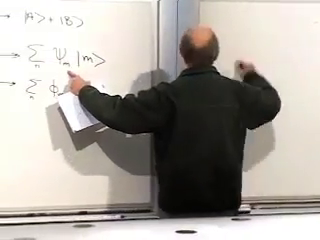
\includegraphics[width=0.68\textwidth]{lecture_07_figure_02.png}
\caption{تفكيكا مساري \(A\) و\(B\) في أساس الشاشة، كلٌّ على حدة.}
\lectureframe{00:05:39}
\end{figure}

إذا أُغلقت \(B\)، فإن الاحتمال عند \(m\) هو
\begin{equation}
P_A(m)=|\psi_m|^2.
\end{equation}
وإذا أُغلقت \(A\)،
\begin{equation}
P_B(m)=|\phi_m|^2.
\end{equation}
كان الاحتمال الكلاسيكي سيقترح جمع هاتين النتيجتين عندما تكون الفتحتان كلتاهما متاحتين. لكن ميكانيكا الكم تجمع السعات أولًا:
\begin{equation}
|A\rangle+|B\rangle
\longrightarrow
\sum_m(\psi_m+\phi_m)|m\rangle.
\end{equation}
وعند موضع ثابت على الشاشة،
\begin{align}
P(m)
&=|\psi_m+\phi_m|^2 \\
&=|\psi_m|^2+|\phi_m|^2
  +\psi_m^*\phi_m+\phi_m^*\psi_m.
\end{align}

\begin{figure}[htbp]
\centering
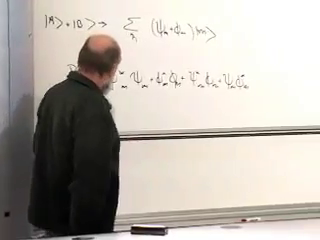
\includegraphics[width=0.70\textwidth]{lecture_07_figure_03.png}
\caption{احتمال الشاشة ذو الحدود الأربعة. والحدان الأخيران هما حدا التداخل.}
\lectureframe{00:09:21}
\end{figure}

عند نقطة تناظر، \(\psi_m=\phi_m\)، ويتعاضد البديلان أحدهما مع الآخر. وعند نقطة تختلف فيها طوراهما بمقدار \(\pi\)، \(\psi_m=-\phi_m\)، ينعدم الاحتمال. يمكن لأي من المسارين وحده أن يصل إلى تلك النقطة، ومع ذلك فإن فتح المسارين معًا قد يمنع الإلكترون من الوصول إليها. والسؤال الآن لا مفر منه: ما الذي يتغير عندما يسجل شيء ما أي الفتحتين استُخدمت؟

\section{يتشابك الكاشف}

أدخل نظامًا مساعدًا ذا حالتين، حالتاه هما \(|u\rangle\) و\(|d\rangle\). وفي هذا النموذج ليس هو لفَّ الإلكترون المغزلي؛ بل هو جهاز خارجي بأبسط صورة ممكنة. في البداية يكون الكاشف غير مُفعَّل:
\begin{equation}
|0,d\rangle.
\end{equation}
رتّب التفاعل بحيث إن المرور عبر \(A\) يقلب حالة الكاشف، في حين أن المرور عبر \(B\) يتركها بلا تغيير:
\begin{equation}
|0,d\rangle
\longrightarrow
|A,u\rangle+|B,d\rangle.
\end{equation}
بعد أن يغادر الإلكترون الفتحتين، لا يعود يتفاعل مع السبين المساعد. ولذلك يتطور الفرعان على النحو
\begin{align}
|A,u\rangle &\longrightarrow \sum_m\psi_m|m,u\rangle, \\
|B,d\rangle &\longrightarrow \sum_m\phi_m|m,d\rangle,
\end{align}
والحالة النهائية هي
\begin{equation}
|\Psi\rangle
=\sum_m\left(\psi_m|m,u\rangle+\phi_m|m,d\rangle\right).
\end{equation}
أصبح المسار وسجل الكاشف الآن متشابكين. وقراءة الكاشف ستكشف أي الفتحتين استُخدمت.

\begin{classroomqa}
\lecturetimestamp{00:13:24}
\audiencequestion{هل انهارت الحزمة الموجية بالفعل حين ينقلب السبين؟}
\lecturerresponse{بالنسبة إلى الإلكترون وحده، يمكن استعمال لغة الانهيار: فبدائل المسار لم تعد تتداخل. أمّا بالنسبة إلى منظومة الإلكترون--الكاشف الكاملة، فلم يُستبعد أي فرع منهما. وما تزال الحالة هي \(|A,u\rangle+|B,d\rangle\). إن تضمين الجهاز يستبدل العبارة \emph{انهار الإلكترون} بالعبارة الدقيقة القائلة إن تشابك المنظومة--الجهاز قد أُقيم.}
\end{classroomqa}

السبين المساعد ليس إلا مؤشرًا مناسبًا. ويمكن لجهاز مُفعَّل أو غير مُفعَّل، أو لفوتون منبعث أو غير موجود، أو لأي زوج آخر من السجلات القابلة للتمييز، أن يؤدي الدور نفسه.

\begin{classroomqa}
\lecturetimestamp{00:15:17}
\audiencequestion{هل يترك المرور عبر الصفيحة المعدنية نفسها دائمًا سجلًا للمسار؟}
\lecturerresponse{ليس بالضرورة. فالمهم هو ما إذا كان التفاعل يترك الصفيحة في حالات نهائية يمكن تمييزها. فإذا كان للصفيحة فجوة إثارة وكان الإلكترون لا يملك طاقة كافية لإثارتها، فلا يلزم أن يترك أثر داخلي دائم. فمجرد التفاعل لا يكفي؛ بل يجب أن يرتبط البديلان بسجلات يمكن تمييزها.}
\end{classroomqa}

\begin{classroomqa}
\lecturetimestamp{00:16:29}
\audiencequestion{هل يمكن أن يكشف ارتداد الصفيحة ما إذا كان الإلكترون قد مر عبر الفتحة العليا أم السفلى؟}
\lecturerresponse{فقط إذا أنتجت دفعتا الزخم المتعاكستان حالتي صفيحة يمكن تمييزهما بدرجة كافية. فالصفيحة المحددة الموضع جيدًا تملك أصلًا دالة موجية واسعة في الزخم. ويمكن للانزياحين الصغيرين إلى أعلى وإلى أسفل أن يتراكبا تقريبًا تراكبًا كاملًا، لذلك فحالـتا الارتداد ليستا متعامدتين ولا توفران سجلًا لا لبس فيه للمسار. وهنا يحمي مبدأ عدم اليقين التداخل.}
\end{classroomqa}

يمكن أن يوجد سجل جزئي. فإذا تلقى الكاشف ركلة طفيفة فقط، فلا يلزم أن تكون حالتا السجل النهائيتان متعامدتين. وعندئذ يُخفَّض التداخل بدلًا من أن يُزال. ولأجل الحساب الصوري نأخذ أولًا الحالة الحدية لقياس كامل:
\begin{equation}
\langle u|d\rangle=0.
\end{equation}

\section{حساب المؤثر المُسقِط}

سنحسب الآن احتمال وصول الإلكترون إلى موضع ثابت على الشاشة هو \(m\)، من دون السؤال عن ناتج الكاشف. وفي فضاء هيلبرت المركب، فإن الخاصية \emph{وجود الإلكترون عند \(m\)} هي فضاء جزئي ثنائي الأبعاد يمتد على
\begin{equation}
|m,u\rangle,\qquad |m,d\rangle.
\end{equation}
والمؤثر المُسقِط الموافق هو
\begin{equation}
\Pi_m
=|m,u\rangle\langle m,u|
 +|m,d\rangle\langle m,d|.
\end{equation}

\begin{figure}[htbp]
\centering
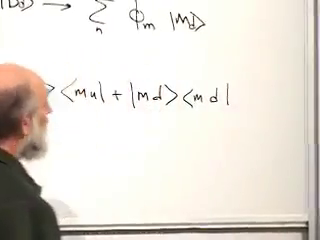
\includegraphics[width=0.66\textwidth]{lecture_07_figure_04.png}
\caption{المؤثر المُسقِط على موضع ثابت على الشاشة، بعد الجمع على سجلي الكاشف المتعامدين.}
\lectureframe{00:22:04}
\end{figure}

تعطي مسلَّمة الاحتمال
\begin{equation}
P(m)=\langle\Psi|\Pi_m|\Psi\rangle.
\end{equation}
وبكتابة المجاميع صراحةً،
\begin{align}
P(m)
&=
\sum_{n,n'}
\left(\psi_n^*\langle n,u|+\phi_n^*\langle n,d|\right)
\notag\\
&\quad\times\Pi_m
\notag\\
&\quad\times
\left(\psi_{n'}|n',u\rangle+\phi_{n'}|n',d\rangle\right).
\end{align}
وتقتضي جداءات الموضع الداخلية \(n=m=n'\). ثم تحدد جداءات الكاشف الداخلية أي الحدود تبقى:
\begin{align}
\langle u|u\rangle&=1,
&
\langle d|d\rangle&=1,
&
\langle u|d\rangle&=\langle d|u\rangle=0.
\end{align}
وعليه،
\begin{equation}
P(m)=|\psi_m|^2+|\phi_m|^2.
\end{equation}

لم تُزَل الحدود المتقاطعة بقرار اعتباطي. إنها تنعدم لأن سعتي المسارين تضربان الآن متجهين متعامدين في فضاء الحالة الموسَّع. ولكي يحدث تداخل، لا بد أن تتفق البدائل لا عند نقطة النهاية على الشاشة فحسب، بل في كل درجة حرية تحمل سجلًا.

\section{ما الذي يُعدّ قياسًا؟}

يوفر نموذج السبين النظيف قاعدة عامة: يحدث القياس حين ينشئ تفاعل ارتباطًا بين بدائل المنظومة وحالات متميزة لجهاز. والتنويعات التالية تختبر هذه القاعدة.

\begin{classroomqa}
\lecturetimestamp{00:26:53}
\audiencequestion{ماذا لو وُضع السبين على نحو متناظر وانقلب عند المرور عبر أيٍّ من الفتحتين؟}
\lecturerresponse{عندئذ يحمل الفرعان السجل نفسه، \(|A,u\rangle+|B,u\rangle=(|A\rangle+|B\rangle)\otimes|u\rangle\). ويمكن فصل حالة الكاشف عاملًا مشتركًا، وهي لا تكشف أي معلومات عن المسار، ولذلك يبقى نمط التداخل.}
\end{classroomqa}

\begin{figure}[htbp]
\centering
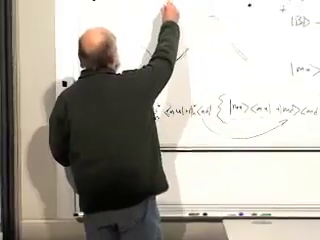
\includegraphics[width=0.68\textwidth]{lecture_07_figure_05.png}
\caption{التنويع المرسوم على اللوح الذي يستجيب فيه كاشف موضوع على نحو متناظر استجابةً متماثلة لكلا المسارين.}
\lectureframe{00:27:14}
\end{figure}

\begin{figure}[htbp]
\centering
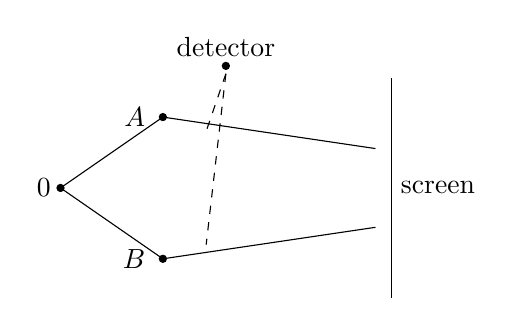
\begin{tikzpicture}[scale=1.0]
\fill (-2,0) circle (1.5pt);
\node[left] at (-2,0) {$0$};
\fill (-0.7,0.9) circle (1.5pt);
\node[left] at (-0.8,0.9) {$A$};
\fill (-0.7,-0.9) circle (1.5pt);
\node[left] at (-0.8,-0.9) {$B$};
\draw (-2,0) -- (-0.7,0.9);
\draw (-2,0) -- (-0.7,-0.9);
\draw (-0.7,0.9) -- (2.0,0.5);
\draw (-0.7,-0.9) -- (2.0,-0.5);
\draw (2.2,-1.4) -- (2.2,1.4);
\node[right] at (2.2,0) {screen};
\fill (0.1,1.55) circle (1.5pt);
\node[above] at (0.1,1.55) {detector};
\draw[dashed] (0.1,1.45) -- (-0.15,0.72);
\draw[dashed] (0.1,1.45) -- (-0.15,-0.72);
\end{tikzpicture}
\caption{إعادة بناء واضحة لوضع الكاشف المتناظر: كلا المسارين ينتجان حالة الكاشف نفسها.}
\end{figure}

\begin{classroomqa}
\lecturetimestamp{00:27:55}
\audiencequestion{هل لا بد أن يقرأ أحدهم السبين المساعد فعلًا قبل أن يختفي التداخل؟}
\lecturerresponse{كلا. فقد ربط الإلكترون بالفعل مساره بالسبين. ويمكن إعادة ضبط الكاشف، وتكرار التجربة إلكترونًا واحدًا في كل مرة، وفحص توزع الإصابات على الشاشة فقط. وتغيب الأهداب حتى إن لم يقرأ أحد السبين؛ فالمهم هو السجل الفيزيائي، لا الوعي البشري به.}
\end{classroomqa}

\begin{classroomqa}
\lecturetimestamp{00:29:36}
\audiencequestion{هل تؤدي صفيحة مرتدة خفيفة بما يكفي إلى تدمير التداخل؟}
\lecturerresponse{نعم، إذا أزاح الارتداد الصفيحة إلى حالتي زخم متعامدتين للمسارين. وإذا ظلت الحزمتان الموجيتان المزاحتان متراكبتين، كان التدمير جزئيًا فقط. وليست الكتلة في حد ذاتها هي المعيار؛ بل قابلية تمييز حالتي الصفيحة النهائيتين.}
\end{classroomqa}

يوفر الإشعاع مسجِّلًا غير كامل آخر. فقد يصدر جسيم مشحون متسارع فوتونًا. وقد لا يكون الإشعاع المنبعث قرب \(A\) هو الحالة نفسها للإشعاع المنبعث قرب \(B\)، ولذلك يمكن للحقل الكهرومغناطيسي أن يحتفظ بمعلومات عن المسار. وبالنسبة إلى إلكترون ينحرف ببطء قد يكون احتمال الانبعاث صغيرًا؛ وتستخدم المحاضرة تقديرًا توضيحيًا يقارب حادثة واحدة من كل مئة. ويجعل التسارع الأقوى الإشعاع، ومن ثم فقدان التباين، أرجح. والنقطة المهمة نوعية: حتى الفوتون غير المرصود يمكنه أن يحمل التماسك بعيدًا.

\begin{classroomqa}
\lecturetimestamp{00:32:00}
\audiencequestion{كيف يُستدل على احتمال التداخل في تجربة حقيقية ذات تباين غير مثالي؟}
\lecturerresponse{تُكرَّر التجربة مرات كثيرة، ويُقدَّر توزيع الشاشة من التكرارات النسبية. وتخلّف العينات المحدودة وسجلات البيئة تسجيلات متبقية في مناطق تُعَدّ مظلمة اسمياً. ويتحسن توزيع الاحتمال المستنتج مع ازدياد عدد المحاولات، بينما تقلل عمليات إزالة الترابط التباين الفيزيائي للأهداب.}
\end{classroomqa}

\begin{classroomqa}
\lecturetimestamp{00:33:13}
\audiencequestion{هل إن أي إمكانية لتحديد المسار تدمر التداخل كله؟}
\lecturerresponse{التمييز التام يقضي عليه تماماً. أما المعلومات الجزئية فتنتج فقداناً جزئياً. فالكاشف الذي لا يُحدِث إلا دوراناً طفيفاً يترك حالتي سجل غير متعامدتين، بحيث يصبح أحد المسارين أرجح من الآخر عند قراءة الكاشف، ولكن من غير يقين؛ وبالمقابل تكون الأهداب مطموسة لا ممحوة.}
\end{classroomqa}

لتدل \(|E_A\rangle\) و \(|E_B\rangle\) على حالتي سجل اعتباطيتين. ويمكن كتابة الحالة المركبة عند الشاشة على الصورة
\begin{equation}
|\Psi\rangle
=\sum_m\left(
\psi_m|m\rangle|E_A\rangle
+\phi_m|m\rangle|E_B\rangle
\right).
\end{equation}
وبإهمال نظام السجل نحصل على
\begin{align}
P(m)
&=|\psi_m|^2+|\phi_m|^2 \\
&\quad
+\psi_m^*\phi_m\langle E_A|E_B\rangle
+\phi_m^*\psi_m\langle E_B|E_A\rangle.
\end{align}
ومن ثم فإن التراكب \(\langle E_A|E_B\rangle\) هو عامل التماسك. فالسجلات المتطابقة تُبقي التداخل كاملاً؛ والسجلات المتعامدة تزيله؛ ويؤدي التراكب المتوسط إلى وضوح متوسط.

\begin{classroomqa}
\lecturetimestamp{00:34:12}
\audiencequestion{إذا انبعثت الفوتونات على فترات متباعدة فقط، فماذا يحدث عندما نحتفظ فقط بأحداث انبعاث الفوتونات؟}
\lecturerresponse{تلك المجموعة الجزئية المنتقاة يكون تداخلها، في الغالب، أضعف لأن الفوتون يحمل معلومات عن المسار. وليس من الضروري أن يكون الفقدان كاملاً: فقد تتراكب حزم موجة الفوتونات المنبعثة عند الفتحتين نفسها، ولذلك قد لا تكون حتى السجلات الإشعاعية متعامدة تماماً.}
\end{classroomqa}

يُوسِّع القصف البيئي نطاق هذه الآلية. فجزيئات الهواء، والفوتونات المحيطة، والمادة المحيطة تكتسب باستمرار سجلات للمواضع العيانية. ولا يبقى شخص أو القمر منتشراً على نحو مرئي في تراكب موضعي متماسك: فالكتلة تبطئ الانتشار الحر، كما أن التشابك البيئي المستمر يكبت التداخل القابل للرصد بين البدائل المنفصلة عيانياً.

\begin{classroomqa}
\lecturetimestamp{00:36:02}
\audiencequestion{أيمثل هذا بالفعل نظرية للقياس، لا مجرد استعمال آخر لعبارة \emph{انهيار حزمة الموجة}؟}
\lecturerresponse{إنها الآلية في مثال مقصود الدقة. ففي وصف يقتصر على الإلكترون، يعني الانهيار حذف الحدود غير القطرية \(\psi^*\phi\). وفي الوصف المركب لا حاجة إلى حذف اعتباطي: فالتشابك مع حالات جهاز متعامدة يجعل تلك الحدود غير متاحة لقياسات تُجرى على الإلكترون وحده. وينبغي رد الأمثلة الأكثر تعقيداً إلى هذه البنية.}
\end{classroomqa}

\begin{classroomqa}
\lecturetimestamp{00:38:04}
\audiencequestion{هل من شأن مجال جاذبي يحني المسار أن يغيّر بطبيعته حجة الإشعاع أو قاعدة التداخل؟}
\lecturerresponse{قد يتغير الإشعاع التفصيلي، وميكانيكا الكم لا تسند مساراً واحداً حاداً قبل قياس المسار. لكن الاستنتاج العام لا يتغير: فالذي يكبت التداخل هو فقط درجة حرية تحتفظ بمعلومات قابلة للتمييز عن المسار. ويجب تحديد جهاز عيني قبل أن يكون للجواب الأكثر تفصيلاً معنى.}
\end{classroomqa}

\begin{classroomqa}
\lecturetimestamp{00:39:44}
\audiencequestion{هل يختلف هذا التداخل عن تداخل الموجات الكهرومغناطيسية الكلاسيكية؟}
\lecturerresponse{في حالة فوتونات كثيرة، يتفق النمط المرصود مع التداخل الموجي المعتاد للمجال الكهرومغناطيسي. وتُظهر تجربة الجسيم المفرد العبارة الكمومية الأعمق: تصل الفوتونات والإلكترونات على هيئة أحداث فردية، بينما تتداخل سعاتها الكمومية. وبالنسبة إلى الإلكترونات، فالموجة المعنية هي دالة موجة الإلكترون، لا موجة كهرومغناطيسية.}
\end{classroomqa}

\begin{classroomqa}
\lecturetimestamp{00:40:45}
\audiencequestion{ماذا يحدث للأجزاء من الموجة الابتدائية الموجَّهة بين \(A\) و \(B\)؟}
\lecturerresponse{في هذا النموذج المتقطع المقصود عمداً، تكون بقية الحاجز محجوبة. فتنعكس تلك الأجزاء ولا تسهم في سعة النفاذ إلى الشاشة. ويعزل النموذج البديلين النافذين من غير ادعاء أن شعاعاً حقيقياً لا يملك إلا مركبتي زخم.}
\end{classroomqa}

\section{القطة، والشاشة، والحدّ الفاصل القابل للتحريك}

تنطبق الرياضيات نفسها على قطة Schr\"odinger. ولتكن للبندقية الحالتان \(|U\rangle\) و \(|F\rangle\) لغير المطلقة والمطلقة، وللقطة الحالتان \(|L\rangle\) و \(|D\rangle\) للحية والميتة. وانطلاقاً من قطة حية وبندقية غير مطلقة، قد يولِّد التفاعل
\begin{equation}
|\Psi_{\mathrm{cat}}\rangle
=\alpha|L,U\rangle+\beta|D,F\rangle.
\end{equation}
والقطة وحدها ليست في الحالة المتماسكة \(\alpha|L\rangle+\beta|D\rangle\). إنها متشابكة مع بندقية سجّلت البديل. والنظر إلى البندقية يمكن أن يكشف فرع القطة، كما أن سجلات البندقية المتعامدة تزيل تداخل الحية--الميتة المعتاد في المنظومة الفرعية للقطة.

\begin{classroomqa}
\lecturetimestamp{00:41:18}
\audiencequestion{هل القطة نفسها في تراكب من كونها حية وميتة؟}
\lecturerresponse{ليس بالمعنى البسيط المعزول. فالنظام المركب القطة--البندقية في تراكب من بدائل مترابطة: حية مع غير مطلقة وميتة مع مطلقة. والمنظومة الفرعية للقطة متشابكة مع بندقية حاملة للسجل، تماماً كما يتشابك مسار الإلكترون مع السبين المساعد.}
\end{classroomqa}

ويجب أيضاً معاملة الشاشة النهائية بوصفها جهازاً. فالإلكترون الواصل إلى \(m\) قد يسوِّد حبيبة فوتوغرافية، أو يجعل مادة وامضة تبعث فوتوناً، أو يقلب حالة كاشف واحد في صف من الأجهزة المحلية ثنائية الحالة. وتصير العلامة مترابطة مع موضع الوصول.

\begin{classroomqa}
\lecturetimestamp{00:43:38}
\audiencequestion{لماذا يجوز لنا أن نتحدث عن احتمالات عند الشاشة النهائية بدلاً من أن نكتفي بمتجهات الحالة إلى الأبد؟}
\lecturerresponse{تسند مسلّمة الاحتمال \(\langle\Pi_m\rangle\) إلى الخاصية \emph{الوصول إلى \(m\)}. ولإكمال التجربة الفيزيائية، تترك الشاشة بعد ذلك سجلاً موضعياً. فالمؤثِّر الإسقاطي يعطي الاحتمال؛ أما اسوداد الحبيبة، أو الوميض، أو انقلاب كاشف موضعي، فيحقق القياس الذي تُجمع إحصاءاته.}
\end{classroomqa}

\begin{classroomqa}
\lecturetimestamp{00:45:00}
\audiencequestion{لماذا نناقش قياساً عند الشاشة، لا احتمالاً للمرور عبر \(A\) أو \(B\)؟}
\lecturerresponse{لا يجوز إسناد احتمالات للمسار واختبارها إلا بتركيب مسجِّل للمسار. ومن دون مثل هذا السجل تبقى البدائل متماسكة ويجب جمعها بوصفها سعات. وعند الشاشة يُفترض وجود جهاز حساس للموضع. والفارق ليس زمناً مميزاً، بل ما إذا كان قد رُتِّب لتفاعل قياس مناظر.}
\end{classroomqa}

يمكن تحريك الحد الفاصل بين النظام والجهاز. أدرج مراقباً له حالتا سجل \(|O_u\rangle\) و \(|O_d\rangle\)؛ فنحصل على
\begin{equation}
|A,u\rangle+|B,d\rangle
\longrightarrow
|A,u,O_u\rangle+|B,d,O_d\rangle.
\end{equation}
ويمكن لمراقب آخر، بدوره، أن يغدو مترابطاً مع الأول. ويمكن أن تُدرج جميعاً في سلسلة تشابك أطول واحدة: الدخان في صندوق القطة، والبندقية، والقطة، Schr\"odinger، وويغنر. وأينما رُسم الحد الفاصل، وجب أن تظل الارتباطات متسقة: فإذا سأل ويغنر لاحقاً Schr\"odinger عما رآه، اتفقت سجلاتهما.

\begin{classroomqa}
\lecturetimestamp{00:47:24}
\audiencequestion{أين بالضبط ينبغي أن ينتهي النظام وأن يبدأ الراصد القائم بالقياس؟}
\lecturerresponse{لا تختار ميكانيكا الكم حداً فاصلاً مناسباً وحيداً. فيمكن للمرء أن يطبّق الانهيار على وصف الإلكترون وحده، أو أن يضم الكاشف ويطبّق الانهيار على وصف أكبر، أو أن يضم مراقباً ويُوسِّع الحالة المتشابكة من جديد. والمقتضى الفيزيائي هو اتساق جميع الاحتمالات والسجلات المتاحة، لا وجود حدّ فاصل وحيد للتدوين الحسابي.}
\end{classroomqa}

\begin{classroomqa}
\lecturetimestamp{00:49:47}
\audiencequestion{هل يدخل مبدأ عدم اليقين لأن قياس المسار يُحدِث اضطراباً في الحدث؟}
\lecturerresponse{نعم. فمثال الارتداد يجعل الصلة صريحة: إذ إن توطين الصفيحة يولِّد لايقيناً في الزخم، ويمكن لذلك أن يمنع الدفعات الصغيرة المعتمدة على المسار من أن تصبح قابلة للتمييز. وعلى نحو أعم، لا يكتمل القياس الكمومي حتى يكون تشابك النظام--الجهاز قد غيّر الحالة، وذلك التغير يمكن أن يبدّل التداخل اللاحق.}
\end{classroomqa}

ويمثل هذا تبايناً حاداً مع المثال الكلاسيكي المثالي. وفي التصور الكلاسيكي يتخيل المرء إمكان إجراء قياس رقيق الأثر إلى حد اعتباطي، واستخراج المعلومات مع اضطراب مهمل. أما هنا فإن استخراج معلومات المسار يقتضي إقامة ارتباط مع جهاز. وهذا تغير حقيقي في الحالة المشتركة، وهو يغير الجواب عن تجربة تداخل لاحقة.

\begin{classroomqa}
\lecturetimestamp{00:52:06}
\audiencequestion{ماذا يحدث إذا أصبح الفصل بين \(A\) و \(B\) كبيراً جداً؟}
\lecturerresponse{لا توجد قاعدة جديدة عامة. ففي هذه الهندسة الخاصة بالمصدر والحاجز قد تصغر ببساطة السعات المؤدية إلى فتحات متباعدة جداً، بحيث تصطدم معظم الجسيمات بالمنطقة المحجوبة. وبصرف النظر عن مثل هذه التغيرات المعتمدة على الجهاز في \(\psi_m\) و \(\phi_m\)، فإن الفصل وحده لا يقرر ما إذا كان التماسك يبقى قائماً.}
\end{classroomqa}

\begin{classroomqa}
\lecturetimestamp{00:53:04}
\audiencequestion{هل خطية التطور الكمي دقيقة تمامًا على المستوى الأساسي، ولماذا تستخدمها الطبيعة؟}
\lecturerresponse{الخطية أساس تجريبي لميكانيكا الكم. ومن المعروف أن إدخال تعديلات لاخطية صغيرة مع الحفاظ على اتساقها المنطقي أمر بالغ الصعوبة، وهي تميل إلى إفساد البنية. أمّا السبب الأعمق لاتباع القضايا الفيزيائية منطق الفضاءات الجزئية بدلًا من المجموعات الكلاسيكية فغير معطى هنا؛ إذ تتعامل المحاضرة معه بوصفه حقيقة من حقائق الطبيعة.}
\end{classroomqa}

\begin{classroomqa}
\lecturetimestamp{00:54:53}
\audiencequestion{هل يمكن لرصد لاحق أن يكشف المسار السابق، ومن ثم يغيّر ما إذا كان التداخل قد حدث؟}
\lecturerresponse{إذا كان بوسع رصد لاحق أن يكشف المسار، فلا بد أن درجة حرية فيزيائية ما قد حفظت سجلًا يعتمد على المسار. وهذا السجل يؤثر بالفعل في التماسك؛ وليس على أحد أن يقرؤه. ويجب مع ذلك احترام السببية، ولا يمكن حسم دعوى مجردة تتعلق بالاختيار المؤجل من دون تحديد الترتيب الكامل في الزمكان والجهاز التجريبي.}
\end{classroomqa}

\begin{classroomqa}
\lecturetimestamp{00:56:47}
\audiencequestion{ماذا لو وُضِعت غرفة فقاعات مباشرة بعد الفتحات؟}
\lecturerresponse{إن أثرًا يميّز بين المسارين الخارجين علامة لا لبس فيها، ولذلك يدمّر التداخل بينهما. وتكفي طبقة رقيقة لتسجيل المسار. وإذا كان جهاز لاحق في مجرى التجربة لا يحتفظ بمعلومات كافية لاستنتاج الفتحة السابقة، فإنه لا يُعد تلقائيًا كاشفًا لأيّ مسار.}
\end{classroomqa}

\begin{classroomqa}
\lecturetimestamp{00:59:29}
\audiencequestion{إذا كان العالم متشابكًا بالفعل بدرجة كبيرة، فكيف يمكن لتجربة تداخل أن تبدأ أصلًا بأنظمة غير متشابكة؟}
\lecturerresponse{يجب أن تعزل عملية التحضير درجات الحرية المعنية، أو تعيد ضبطها، أو تكيّفها بما يكفي بحيث تبدأ البدائل بالسجل البيئي نفسه. ولا يمكن ببساطة تجاهل أثر سابق في غرفة فقاعات إذا ظل مترابطًا مع المسار. فالتداخل يتطلب علاقة ابتدائية شبيهة بحالة الجداء بين النظام المتحكَّم فيه والمسجِّل المعني.}
\end{classroomqa}

\begin{classroomqa}
\lecturetimestamp{01:01:04}
\audiencequestion{من أين يأتي فك التشابك العملي بعد القياس؟}
\lecturerresponse{باشتراط نتيجة مرصودة محددة. فإذا وُجد اللفّ المغزلي إلى أعلى، احتفظ الراصد بالفرع \(|A,u\rangle\) وحذف البديل من الوصف العملي. ويمكن استخدام حالة الجداء الشرطية تلك نقطةَ بداية جديدة. وقد تبقى الحالة الكاملة الشاملة للراصد متشابكة، لكن التحضير المختار يكون محددًا بالنسبة إلى النتيجة المسجَّلة.}
\end{classroomqa}

هذا التسلسل الهرمي المتداخل لا يحل كل سؤال تأويلي، لكنه يُظهر الاتساق العملي. ويمكن أن يشمل النظام والكاشف والراصد وراصدَ الراصد جميعًا. وأيًّا كان الموضع الذي يُقطَع عنده الوصف، فإن السجلات المترابطة على نحو صحيح لا تتناقض لاحقًا بعضها مع بعض.

\section{من التشابك إلى الإنتروبيا}

لقد مضى النقاش في موضوع القياس أبعد مما كان مخططًا، لكنه أبرز السؤال التالي: كيف يمكن قياس درجة التشابك؟
لفّان مغزليان في حالة الجداء
\begin{equation}
|u\rangle\otimes|u\rangle
\end{equation}
ليسا متشابكين. فلكل منظومة فرعية حالتها المحددة الخاصة بها، ورصد إحداهما لا يزوّد بأي معلومات جديدة عن الأخرى. أما الحالات المتشابكة فلا تنحلّ إلى جداء على هذا النحو. وسيكون المعيار الكمي القياسي هو إنتروبيا التشابك، لكننا نحتاج أولًا إلى المفهوم العادي للإنتروبيا ثم إلى صورتها الكمية.

\section{الإنتروبيا الكلاسيكية بوصفها معلومات مفقودة}

ابدأ بنظام كلاسيكي له مجموعة منتهية من \(N\) حالات ممكنة. الإنتروبيا هنا خاصية للنظام مقترنة بمعرفتنا به. افترض أن كل ما نعرفه هو أن النظام يشغل واحدة من \(n\) حالات متساوية الاحتمال. عندئذ
\begin{equation}
S=\log n.
\end{equation}
إذا كان \(n=1\)، فالحالة معروفة و\(S=0\). وإذا كان \(n=N\)، فلا يُعرف شيء يتجاوز فضاء الحالات نفسه، وتكون الإنتروبيا عظمى، \(S_{\max}=\log N\).

يحصي اللوغاريتم اختيارات نعم--لا المستقلة على نحوٍ إضافي. بالنسبة إلى \(M\) لفّات مغزلية كلاسيكية، توجد \(2^M\) تهيئة، ومن ثم
\begin{equation}
\log(2^M)=M\log 2.
\end{equation}
وبغض النظر عن اختيار أساس اللوغاريتم، فإن الإنتروبيا بذلك تحصي مقدار المعلومات الثنائية المفقودة من الوصف.

أما لتوزيع احتمالي عام \(p_i\)، فالتعريف المناسب هو
\begin{equation}
S=-\sum_i p_i\log p_i.
\end{equation}

\begin{classroomqa}
\lecturetimestamp{01:14:17}
\audiencequestion{لماذا توجد إشارة سالبة في صيغة الإنتروبيا؟}
\lecturerresponse{كل احتمال غير صفري يحقق \(0<p_i\leq 1\)، ومن ثم \(\log p_i\leq 0\). وتجعل الإشارة السالبة الإنتروبيا غير سالبة. وعند \(p_i=0\)، يُعرَّف الإسهام بالحد \(p_i\log p_i\to0\).}
\end{classroomqa}

بالنسبة إلى توزيع تساوي الاحتمالات
\begin{equation}
p_i=
\begin{cases}
1/n, & i\in\mathcal N,\\
0, & i\notin\mathcal N,
\end{cases}
\qquad |\mathcal N|=n,
\end{equation}
تصبح الصيغة العامة
\begin{align}
S
&=-n\left(\frac1n\right)\log\left(\frac1n\right)\\
&=\log n.
\end{align}
ولذلك فهي تعيد إنتاج تعريف العدّ الابتدائي. أما التوزيع المتركز يقينًا على حالة واحدة فله \(S=0\).

\begin{figure}[htbp]
\centering
\includegraphics[width=0.66\textwidth]{lecture_07_figure_07.png}
\caption{يعرض اللوح \(S=\log n\)، وصيغة شانون، والتحقق في حالة تساوي الاحتمالات.}
\lectureframe{01:16:08}
\end{figure}

\begin{classroomqa}
\lecturetimestamp{01:17:35}
\audiencequestion{ما أكبر إنتروبيا يمكن أن تكون لنظام له \(N\) حالة، وما الذي يكون معلومًا عندئذ؟}
\lecturerresponse{القيمة العظمى هي \(\log N\)، وتتحقق عند التوزيع المنتظم \(p_i=1/N\). ومع ذلك يبقى معلومًا ما هو النظام، ومن ثم يُعرف فضاء حالاته؛ والمجهول هو أيَّ حالة من تلك \(N\) الحالات يشغلها.}
\end{classroomqa}

والفرق
\begin{equation}
I=S_{\max}-S
\end{equation}
هو المعلومات المتاحة بهذا المعنى العدّي. والإنتروبيا والمعلومات وجهان متقابلان للسجل الحسابي نفسه: فالإنتروبيا تسجل المعلومات التي كان يمكن أن تميّز الحالة ولكنها غير متاحة لنا.

\section{الأثر: البديل الكمي للجمع}

بالنسبة إلى مؤثر \(M\) وأي أساس متعامد متطبع كامل \(\{|i\rangle\}\)، نعرّف
\begin{equation}
\operatorname{Tr}M
=\sum_i\langle i|M|i\rangle.
\end{equation}

\begin{figure}[htbp]
\centering
\includegraphics[width=0.68\textwidth]{lecture_07_figure_08.png}
\caption{الأثر مكتوبًا على صورة مجموع العناصر القطرية للمصفوفة.}
\lectureframe{01:21:20}
\end{figure}

مع أن التعريف مكتوب باستخدام أساس، فإن النتيجة مستقلة عن الأساس. وبالنسبة إلى مؤثر هيرميتي يمكن اختيار أساس ذاتي، وعنده
\begin{equation}
\operatorname{Tr}M=\sum_i\lambda_i.
\end{equation}
فالقيم الذاتية، ومن ثم مجموعها، لا تعتمد على الإحداثيات المستخدمة لتمثيل المؤثر.

\begin{classroomqa}
\lecturetimestamp{01:23:04}
\audiencequestion{هل يقتضي وضع مصفوفة في صورة قطرية أن تكون لها معكوسة؟}
\lecturerresponse{لا. فالصورة القطرية تُظهر القيم الذاتية؛ أمّا القابلية للعكس فشرط منفصل. وتكون المصفوفة القطرية قابلة للعكس على وجه التحديد عندما لا تكون أيّ من قيمها الذاتية القطرية صفرًا. ويمكن وضع المصفوفات الهيرميتية في صورة قطرية حتى عندما تنعدم بعض القيم الذاتية.}
\end{classroomqa}

بعد الاستراحة، نعود بإيجاز إلى الاحتمال الكلاسيكي. الكمية المرصودة الكلاسيكية هي دالة \(f_i\) للتهيئة، ومتوسطها هو
\begin{equation}
\langle f\rangle_{\mathrm{cl}}=\sum_i p_i f_i.
\end{equation}
وفي الصيغ الكمية، سيحل الأثر محل المجموع على البدائل، وسيحل مؤثر محل الدالة الكلاسيكية، وستحل مصفوفة كثافة محل التوزيع الاحتمالي.

\section{المخاليط الإحصائية ومصفوفة الكثافة}

افترض أن شخصًا ما يحضّر نظامًا في إحدى حالات أساس متعامد متطبع، لكنه لا يخبرنا أيَّ حالة اختيرت. ولا يعطوننا إلا احتمالات التحضير---فعلى سبيل المثال، يُحضَّر لفّ مغزلي إلى أعلى باحتمال \(3/4\) وإلى أسفل باحتمال \(1/4\). وهذا ليس التراكب المتماسك
\begin{equation}
\sqrt{\frac34}|u\rangle+\sqrt{\frac14}|d\rangle,
\end{equation}
لأنه لم يُحضَّر أي طور نسبي. بل هو خليط إحصائي من حالات محددة. وتبقى الاحتمالات الكمية قائمة حتى عندما تكون الحالة النقية معلومة؛ وهنا توجد لايقينية إضافية بشأن أي حالة نقية جرى تحضيرها.

\begin{figure}[htbp]
\centering
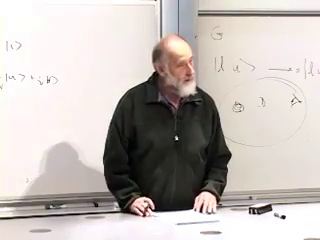
\includegraphics[width=0.66\textwidth]{lecture_07_figure_06.png}
\caption{الانتقال المفهومي من كيت محدد إلى وصف لمجموعة إحصائية.}
\lectureframe{01:29:43}
\end{figure}

إذا جرى تحضير الحالة \(|i\rangle\) باحتمال \(\rho_i\)، فإن مؤثر الكثافة هو
\begin{equation}
\rho=\sum_i\rho_i|i\rangle\langle i|.
\end{equation}
وفي أساس التحضير،
\begin{equation}
\rho=
\begin{pmatrix}
\rho_1&0&0&\cdots\\
0&\rho_2&0&\cdots\\
0&0&\rho_3&\cdots\\
\vdots&\vdots&\vdots&\ddots
\end{pmatrix}.
\end{equation}

\begin{figure}[htbp]
\centering
\includegraphics[width=0.68\textwidth]{lecture_07_figure_09.png}
\caption{مصفوفة الكثافة القطرية وشرط تطبيعها.}
\lectureframe{01:32:12}
\end{figure}

قيمها الذاتية حقيقية وغير سالبة، ويصبح تطبيع الاحتمالات
\begin{equation}
\operatorname{Tr}\rho=\sum_i\rho_i=1.
\end{equation}

لتكن \(F\) كمية مرصودة هيرميتية. فقيمة التوقع للمجموعة الإحصائية هي
\begin{equation}
\langle F\rangle=\operatorname{Tr}(F\rho).
\end{equation}

\begin{figure}[htbp]
\centering
\includegraphics[width=0.68\textwidth]{lecture_07_figure_10.png}
\caption{قيمة التوقع المعبر عنها بالأثر \(\langle F\rangle=\operatorname{Tr}(F\rho)\).}
\lectureframe{01:35:05}
\end{figure}

ولاسترجاع المتوسط الموزون المعتاد، احسب الأثر في الأساس الذي تكون فيه \(\rho\) قطرية، وأدرج تحليل الوحدة:
\begin{align}
\operatorname{Tr}(F\rho)
&=\sum_i\langle i|F\rho|i\rangle\\
&=\sum_{i,j}\langle i|F|j\rangle
               \langle j|\rho|i\rangle\\
&=\sum_i\rho_i\langle i|F|i\rangle.
\end{align}
وهكذا تُوزَن قيمة التوقع لكل حالة نقية باحتمال تحضير الحالة المناظرة.

وللأثر الخاصية الدورية
\begin{equation}
\operatorname{Tr}(AB)=\operatorname{Tr}(BA),
\end{equation}
حتى إذا كان \(A\) و\(B\) لا يتبادلان. ومن ثم \(\operatorname{Tr}(F\rho)=\operatorname{Tr}(\rho F)\).

\section{الإنتروبيا الكمية والعائد المؤجَّل}

إنتروبيا مصفوفة الكثافة هي
\begin{equation}
S(\rho)=-\operatorname{Tr}(\rho\log\rho).
\end{equation}
وبالنسبة إلى مؤثر هيرميتي موجب، تُعرَّف دوال من قبيل \(\log\rho\) عبر قيمه الذاتية. فإذا كان
\begin{equation}
\rho=\sum_i\rho_i|i\rangle\langle i|,
\end{equation}
فعندئذ
\begin{equation}
\log\rho=\sum_{\rho_i>0}(\log\rho_i)|i\rangle\langle i|,
\end{equation}
ومن ثم
\begin{equation}
S(\rho)=-\sum_i\rho_i\log\rho_i.
\end{equation}

\begin{figure}[htbp]
\centering
\includegraphics[width=0.68\textwidth]{lecture_07_figure_11.png}
\caption{صيغة الإنتروبيا الكلاسيكية بعد إعادة كتابتها على الصورة \(S=-\operatorname{Tr}(\rho\log\rho)\).}
\lectureframe{01:41:25}
\end{figure}

للحالة النقية المعروفة مؤثر الكثافة
\begin{equation}
\rho_\psi=|\psi\rangle\langle\psi|,
\end{equation}
وقيمه الذاتية هي \(1,0,\ldots\)، ومن ثم \(S(\rho_\psi)=0\). وهذا لا يعني أن لكل قياس على \(|\psi\rangle\) ناتجًا مؤكدًا. بل يعني أنه لا يوجد جهل إحصائي إضافي بشأن الحالة المُحضَّرة. وعلى الطرف المقابل تمامًا،
\begin{equation}
\rho=\frac{I}{d}
\qquad\Longrightarrow\qquad
S(\rho)=\log d,
\end{equation}
حيث \(d=\dim\mathcal H\). وتُسنِد الحالة المختلطة العظمى وزنًا متساويًا إلى كل اتجاه متعامد.

أصبحت الصلة بالتشابك الآن قريبة، لكنها لم تُستكمل بعد. افترض أن نظامًا مركبًا \(AB\) في حالة مشتركة، وأن جميع التجارب مقتصرة على \(A\). لا بد من وجود كائن يعيد إنتاج كل قيمة توقّع يمكن الحصول عليها على \(A\) مع تجاهل \(B\). وهذا الكائن هو مصفوفة كثافة لـ \(A\). وإذا كانت الحالة المشتركة تتفكك إلى حاصل ضرب، فإن مصفوفة الكثافة الخاصة بـ \(A\) تكون نقية وذات إنتروبيا صفرية. وإذا كان \(A\) و\(B\) متشابكين، فإن مصفوفة الكثافة الخاصة بـ \(A\) تكون عمومًا مختلطة وذات إنتروبيا غير صفرية. وإنشاء مصفوفة الكثافة المختزلة تلك وحساب إنتروبيتها هو المهمة المؤجَّلة إلى المحاضرة التالية.